\documentclass{bmcart}

%%% Load packages
%\usepackage{amsthm,amsmath}
\usepackage{amsmath}
\usepackage{setspace}
\usepackage{lineno}
\usepackage{url}
\linenumbers
\RequirePackage[sort]{natbib}
%\RequirePackage[authoryear]{natbib}% uncomment this for author-year bibliography
%\RequirePackage{hyperref}
\usepackage[utf8]{inputenc} %unicode support
%\usepackage[applemac]{inputenc} %applemac support if unicode package fails
%\usepackage[latin1]{inputenc} %UNIX support if unicode package fails
\usepackage{graphicx}
% \def\includegraphic{}
% \def\includegraphics{}


\startlocaldefs
\endlocaldefs


%%% Begin ...
\begin{document}

%\setcounter{page}{0}  %% ugh, article template assumes starting on odd page!
% \newpage

%%% Start of article front matter
\begin{frontmatter}

\begin{fmbox}
\dochead{Research}

%% TO DO
% author references (maybe fix programmatically?)
% acknowledgments

%%%%%%%%%%%%%%%%%%%%%%%%%%%%%%%%%%%%%%%%%%%%%%
%%                                          %%
%% Enter the title of your article here     %%
%%                                          %%
%%%%%%%%%%%%%%%%%%%%%%%%%%%%%%%%%%%%%%%%%%%%%%

\title{Incorporating Periodic Variability in Hidden Markov Models for Animal Movement}

%%%%%%%%%%%%%%%%%%%%%%%%%%%%%%%%%%%%%%%%%%%%%%
%%                                          %%
%% Enter the authors here                   %%
%%                                          %%
%% Specify information, if available,       %%
%% in the form:                             %%
%%   <key>={<id1>,<id2>}                    %%
%%   <key>=                                 %%
%% Comment or delete the keys which are     %%
%% not used. Repeat \author command as much %%
%% as required.                             %%
%%                                          %%
%%%%%%%%%%%%%%%%%%%%%%%%%%%%%%%%%%%%%%%%%%%%%%

\author[
   addressref={aff1},                   % id's of addresses, e.g. {aff1,aff2}         
   email={lim88@mcmaster.ca}   % email address
]
{\inits{ML}\fnm{Michael} \snm{Li}}
\author[
   addressref={aff1,aff2},
   email={bolker@mcmaster.ca}
]{\inits{BMB}\fnm{Benjamin M.} \snm{Bolker}}

%%%%%%%%%%%%%%%%%%%%%%%%%%%%%%%%%%%%%%%%%%%%%%
%%                                          %%
%% Enter the authors' addresses here        %%
%%                                          %%
%% Repeat \address commands as much as      %%
%% required.                                %%
%%                                          %%
%%%%%%%%%%%%%%%%%%%%%%%%%%%%%%%%%%%%%%%%%%%%%%

\address[id=aff1]{                            % unique id
  \orgname{Department of Biology, McMaster University}, % university, etc
  \street{1280 Main St. West},                     %
  \postcode{L8S 4K1},                                % post or zip code
  \city{Hamilton, Ontario},                              % city
  \cny{Canada}                                    % country
}
\address[id=aff2]{
  \orgname{Department of Mathematics and Statistics, McMaster University},
  \street{1280 Main St. West},
  \postcode{L8S 4K1},
  \city{Hamilton, Ontario},
  \cny{Canada}
}

%%%%%%%%%%%%%%%%%%%%%%%%%%%%%%%%%%%%%%%%%%%%%%
%%                                          %%
%% Enter short notes here                   %%
%%                                          %%
%% Short notes will be after addresses      %%
%% on first page.                           %%
%%                                          %%
%%%%%%%%%%%%%%%%%%%%%%%%%%%%%%%%%%%%%%%%%%%%%%

\begin{artnotes}
% \note{Sample of title note}     % note to the article
% \note[id=n1]{Equal contributor} % note, connected to author
\end{artnotes}

\end{fmbox}% comment this for two column layout

%%%%%%%%%%%%%%%%%%%%%%%%%%%%%%%%%%%%%%%%%%%%%%
%%                                          %%
%% The Abstract begins here                 %%
%%                                          %%
%% Please refer to the Instructions for     %%
%% authors on http://www.biomedcentral.com  %%
%% and include the section headings         %%
%% accordingly for your article type.       %%
%%                                          %%
%%%%%%%%%%%%%%%%%%%%%%%%%%%%%%%%%%%%%%%%%%%%%%

\begin{abstractbox}

\begin{abstract} % abstract


%% need to break into background, 

% More generally, we point out that model misspecification
% (omitting important sources of variation) can lead to overfitting,
% and as a corollary that incorporating previously neglected
% structure in statistical models can allow more
% accurate assessment of appropriate model complexity.

\parttitle{Background} %if any
Clustering time-series data into discrete groups can improve 
prediction and provide insight into the nature of underlying,
unobservable states of the system. However, temporal variation in the
rates at which individuals move between groups can obscure
such signals. We use finite mixture and hidden Markov models (HMMs), two
standard clustering techniques, to model high-resolution hourly
movement data from Florida panthers (\emph{Puma concolor coryi}).
Allowing for temporal heterogeneity in transition probabilities, a straightforward 
but little-used extension of the standard HMM framework, 
resolves some shortcomings of current
models and clarifies the behavioural patterns of
panthers.

\parttitle{Results} %if any
Simulations and Florida panthers data showed model misspecification (omitting important 
sources of variation) can lead to overfitting and over-estimating number of behavioural states. Models incorporating temporal heterogeneity have lower number of states with slightly higher variation in short movement states, and able to make out of sample predictions that captures observed diurnal and autocorrelation patterns exhibited by Florida panthers.     

\parttitle{Conclusion} %if any
Incorporating temporal heterogeneity reduce the selected number of behavioural states closer 
to a biologically interpretable level, improved goodness of fit and predictability. Our 
suggest that incorporating previously neglected structure in statistical models can
allow more accurate assessment of appropriate model complexity.

\end{abstract}

%%%%%%%%%%%%%%%%%%%%%%%%%%%%%%%%%%%%%%%%%%%%%%
%%                                          %%
%% The keywords begin here                  %%
%%                                          %%
%% Put each keyword in separate \kwd{}.     %%
%%                                          %%
%%%%%%%%%%%%%%%%%%%%%%%%%%%%%%%%%%%%%%%%%%%%%%

\begin{keyword}
\kwd{Hidden Markov Model}
\kwd{Animal Movement}
\kwd{Temporal Autocorrelation}
\kwd{Temporal Heterogeneity}
\kwd{Florida Panther}
\end{keyword}

% MSC classifications codes, if any
%\begin{keyword}[class=AMS]
%\kwd[Primary ]{}
%\kwd{}
%\kwd[; secondary ]{}
%\end{keyword}

\end{abstractbox}
%
%\end{fmbox}% uncomment this for twcolumn layout

\end{frontmatter}

%%%%%%%%%%%%%%%%%%%%%%%%%%%%%%%%%%%%%%%%%%%%%%
%%                                          %%
%% The Main Body begins here                %%
%%                                          %%
%% Please refer to the instructions for     %%
%% authors on:                              %%
%% http://www.biomedcentral.com/info/authors%%
%% and include the section headings         %%
%% accordingly for your article type.       %%
%%                                          %%
%% See the Results and Discussion section   %%
%% for details on how to create sub-sections%%
%%                                          %%
%% use \cite{...} to cite references        %%
%%  \cite{koon} and                         %%
%%  \cite{oreg,khar,zvai,xjon,schn,pond}    %%
%%  \nocite{smith,marg,hunn,advi,koha,mouse}%%
%%                                          %%
%%%%%%%%%%%%%%%%%%%%%%%%%%%%%%%%%%%%%%%%%%%%%%

%%%%%%%%%%%%%%%%%%%%%%%%% start of article main body
% <put your article body there>

%%%%%%%%%%%%%%%%
%% Background %%
%%
% \section*{Content}
% Text and results for this section, as per the individual journal's instructions for authors. %\cite{koon,oreg,khar,zvai,xjon,schn,pond,smith,marg,hunn,advi,koha,mouse}

\doublespacing

\section*{Background}

Given a sequence of animal movements, movement models aim to find a parsimonious description
that can be used to understand past movements and predict
future movements. Ecologists have long considered the effects of
individual-level covariates (sex, age, nutritional status) and
environmental covariates (habitat type, location of predators or prey)
on movement \cite{patterson2008state, mckenzie2009first, pal1998dispersal}. 
More recently, modelers have developed
\emph{hidden Markov models} (HMMs)
\cite{firle_influence_1998,nathan_movement_2008,langrock_flexible_2012} % 
--- used in animal ecology under the rubric of the ``multiphasic movement
framework'' \cite{fryxell_multiple_2008} --- that consider the effects
of organisms' \emph{internal} states; in particular, HMMs model animal
movement as though individual animals' movement behaviour 
at particular times is determined
by which of a discrete set of unobserved movement states
(e.g. ``foraging'', ``traveling'', ``resting'') they currently occupy.
Conditional on the state occupied by an individual, HMMs typically
assume that animals follow a standard correlated walk model
\cite{okubo_diffusion_1980,turchin1998quantitative}.


Ever-increasing capabilities of remote
sensors are making movement data available over an
ever-wider range of time scales, at both higher resolution (e.g. hourly data
from GPS collars vs. daily or weekly fixes for radio or VHF
collars) and longer extent (e.g. from a few days to significant
fractions of a year, or longer).  When analyzing such
long-term data, ecologists will more
often have to account for temporal variability in movement
behaviour at diurnal and seasonal scales that were previously
not captured in the data.


HMMs have typically been used to model movements over short time
scales, where the probability of transitioning between movement states is
approximately constant. Changes in latent/hidden behavioural state/mode transition 
% BMB: pick one (perhaps include a parenthetical statement/definition
% saying that we treat these as a synonyms.  Just stringing them together
% with slashes is awkward)
probabilities based on
the local environment can be accounted for incorporating environmental
covariates in the HMM \cite{patterson_classifying_2009}, or by more
direct comparisons between inferred states and environmental
conditions \cite{fryxell_multiple_2008}. Schliehe-Diecks et al. 
\cite{schliehe-diecks_application_2012}
consider temporal trends in behavioural transitions over the
time scales of a six-hour
observation period, but
in general ecologists have turned to other tools to describe behavioural
changes over longer (diurnal, seasonal, or ontogenetic) time scales \cite{gurarie2009novel}.


For movement behaviours that change on a fast time scale, such
that movement behaviours recorded
at successive observations are effectively independent,
\emph{finite mixture models} (FMMs) --- which can be considered
a special case of HMMs where the
probability of state occupancy is independent of the previous state ---
can adequately describe movement \cite{tracey_mapping_2012}.  
When movement varies over long time scales
(relative to the time between observations) with little short-term
persistence or correlation, movement could be well represented by FMMs
where the occupancy probabilities change deterministically over time.
Thus FMMs and HMMs,
with or without temporal variation in the occupancy or transition
probabilities, form a useful family of models for capturing
changes in movement behaviour over a range of time scales.


Our primary goal in this paper is to introduce the use of
HMMs with temporally varying transition probabilities -- in particular,
transition probabilities that follow a diurnal cycle -- for modeling
animal movement recorded over long time scales.  
In addition to simulation-based examples,
we also re-analyze data from 
van de Kerk et al. \cite{kerk2015hidden}, who used temporally homogeneous hidden semi-Markov
models (HSMMs: an extension of HMMs that allow
flexible modelling of the distribution of \emph{dwell times}, the 
lengths of consecutive occupancy of a behavioural state) to
describe the movement and putative underlying
behavioural states of Florida panthers (\emph{Puma concolor coryi}).

van de Kerk et al. \cite{kerk2015hidden} found that the best-fitting HSMMs
incorporated a surprisingly large number of hidden
behavioural states (as many as six for individuals with a large amount
of available data); for reasons of computational 
practicality and biological interpretability, they restricted their
detailed analysis to models with only three underlying states.  In
contrast, most studies using HMM have chosen the
number of underlying states \emph{a priori}, typically using either two
\cite{schliehe-diecks_application_2012,mckellar_using_2014,langrock_flexible_2012,fryxell_multiple_2008}, or three states
\cite{dean2012behavioural,morales_extracting_2004,franke_prediction_2006}. 
In contrast, \cite{dean_behavioural_2013} evaluated models with up to 10
states, but like \cite{kerk2015hidden} they chose to consider only 
models with three states. 
As van de Kerk et al. \cite{kerk2015hidden} comment, and as
we discuss further below, behavioural
repertoires with more than three distinct states are difficult to
interpret --- one possible reason that other authors have not adopted
van de Kerk et al.'s model-based approach to
identifying the number of latent states.

Our second goal, therefore, is to explore whether
van de Kerk et al.'s results on optimal
model complexity might be driven at
least in part by structural problems with their statistical
model, i.e. the
assumption of temporally homogeneous behaviour.  For large data sets, 
information-theoretic model selection methods will
typically choose complex, highly parameterized models; when there is
only one way in which models can become more complex (e.g. by
increasing the number of latent states), complexity that is
present in the data but not accounted for in the model (e.g. spatial
or temporal heterogeneity) can be misidentified as other forms of
complexity.  We predict that increasing volumes of data will
increasingly lead researchers who are accustomed to fitting 
small models to sparse data into such traps.  We examine whether
allowing for diurnal variation in the Florida panther data leads to
selection of models with smaller numbers of latent states; we also
fit models to simulated data with varying numbers of latent states
and degrees of temporal heterogeneity to test our conjecture that
heterogeneity can be misidentified as behavioural complexity.

\section*{Methods}

\subsection*{Data and previous analyses}


GPS collars were fitted to 18 Florida panthers in 2005-2012 by Florida
Fish and Wildlife and Conservation Commission staff using
trained hounds and houndsmen. Of these animals, 13 had 
sufficient data to be used by van de Kerk et al. \cite{kerk2015hidden}.
Here we focus on the four cats with the most data (all with approximately 10,000-15,000
observations: see Table~1), 
in part because our goal is to understand
the issues that arise when simple models are fitted to large data sets, and 
in part because the general trend in telemetry studies is toward larger data sets.  
As is typical in studies of animal movement, 
we took first differences of the data by decomposing
contiguous sequences of hourly GPS coordinates into 
successive step lengths (in meters) and turning angles (in radians)
\cite{turchin1998quantitative,kerk2015hidden}.


van de Kerk et al. \cite{kerk2015hidden} used hidden semi-Markov models (HSMM), 
an extension of HMM that permits explicit modelling of dwell times 
\cite{langrock_flexible_2012}, considering both Poisson and
negative binomial distributions for dwell times.  As shown 
by van de Kerk et al. \cite{kerk2015hidden} (Figure S3b, top row, middle panel),
the estimated shape parameter of the negative binomial dwell time
distribution was typically close to 1 ($\approx 0.4-1.6$; confidence
intervals were not given), implying that a geometric distribution
(i.e., negative binomial with shape=1) might be adequate. In turn,
this suggests that we might not lose much accuracy by reverting to 
a simpler HMM framework, which corresponds
to making precisely this assumption.


van de Kerk et al. \cite{kerk2015hidden} considered time-homogeneous models with 
a variety of candidate distributions %
--- log-Normal, Gamma, and Weibull distributions for step lengths
and von Mises and wrapped Cauchy distributions for the turning angle --- %
concluding on the basis of the Akaike information criterion (AIC) 
that Weibull step length and wrapped Cauchy turning angle distributions
were best.  
Since our analysis aims for simplicity and qualitative
conclusions rather than for picking the very best
predictive model, we focus on models that treat each step as
a univariate, log-Normally distributed observation, glossing
over both the differences in shape between
the three candidate step-length distributions and the effects
of considering multivariate (i.e., step length plus turning angle)
observations.  However, we do briefly compare log-Normal and Weibull
step-length distributions, with and without 
a von Mises-distributed turning angle included in the model (Figure 2).
(Note that most movement analyses, including van de Kerk et al.
\cite{kerk2015hidden}, are only partially multivariate, 
treating step length and turning angle at a particular time
as multivariate observations for the purpose of HMM
analysis but neglecting possible correlations
between the two measures.) 


van de Kerk et al. \cite{kerk2015hidden} used the Bayesian (Schwarz) information criterion (BIC)
to test the relative penalized goodness of fit for
models ranging from 2 to 6 latent states.
In general, BIC values decreased as the number of states
increased from 
three to six states,
suggesting that the six-state model was
favoured statistically; however,
the authors used three-state models in most
of their analyses for ease of biological interpretation.
We follow van de Kerk et al. \cite{kerk2015hidden} in using BIC-optimality (i.e., minimum
BIC across a family of models) as the criterion for identifying
the best model, because we are interested in explaining the 
data generation process by identifying the ``true'' number 
of underlying movement states.  

Using BIC also simplifies 
evaluation of model selection procedures; 
it is easier to test whether our model selection
procedure has selected the model used to simulate the data,
rather than testing whether it has selected the model with
the minimal Kullback-Leibler distance
\cite{Richards2005}. We recognize that 
ecologists will often be interested in maximizing predictive
accuracy rather than selecting a true model, and that as
usual in ecological systems the true model will be far more
complicated than any candidate model \cite{BurnhamAnderson1998};
we believe that the qualitative conclusions stated here
for BIC-optimality will carry over to analyses using AIC instead.

\subsection*{Model description}

\newcommand{\obs}{\mathbf{y}}
\newcommand{\cov}{\mathbf{x}}
\newcommand{\state}{z}

In a HMM, the joint likelihood of \emph{emissions} (i.e., direct observations) $ \mathbf Y = \obs_{1},..., \obs_{T}$ 
and a hidden state sequence $\mathbf{Z}, \state_{t} \in \{1,...,n\}, t=1,...,T$, given model
parameters {\boldmath $\theta$} and covariates $\mathbf{X}_{1:T} =\cov_{1},..., \cov_{T}$, can be written as:

\begin{equation}
\begin{split}
P(\mathbf{Y}_{1:T},\mathbf{Z}_{1:T}|\boldsymbol \theta,\mathbf{X}_{1:T}) & =
P(\state_{1} \mid \cov_{1})P(\obs_{1} | \state_{1}, \cov_{1}) \cdot \\
&  \quad \prod\limits_{k=2}^{T}P(\state_{k} | \state_{k-1}, \cov_{k})P(\obs_{k} | \state_{k},\cov_{k})
\end{split}
\label{eq:HMMlik}
\end{equation}

The emissions $\obs_i$ are boldfaced to denote that we may have a vector of observations at each time point (e.g., step length and turning angle).
The model contains three distinct components:

\begin{description}
\item[Initial probability] $P(\state_{1} = i | \cov_{1}) P(\obs_{1} | \state_{1}, \cov_{1} )$: the probability of state $i$ at time $t=1$ where the covariate is $\cov_{1}$, times the vector of observations $\obs_{1}$ conditioned on covariates $\cov_{1}$ and state $\state_{1}$.


\item[Transition probability] $P(\state_{k}=j | \state_{k-1}=i,\cov_{k})$: the probability of a transition from state $i$ at time $t=k-1$ to state $j$ with covariate $\cov_{k}$ at time $t=k$.


\item[Emission probability] $P(\obs_{k} | \state_{k},\cov_{k})$: a vector of observations $\obs_{k}$ conditioned on covariates $\cov_{k}$ at state $\state_{k}$ at time $t=k$.  
\end{description}

Eq.~\ref{eq:HMMlik} gives the likelihood of the observed sequence 
given (conditional on) a particular
hidden sequence. 
In order to calculate the overall, unconditional (or marginal) 
likelihood of the 
observed sequence, we need to average over all possible hidden sequences. 
There are several efficient algorithms for computing the marginal likelihood and
numerically estimating parameters \cite{zucchini_hidden_2009};
we used those implemented in the \texttt{depmixS4} package for R
\cite{visser2010depmixs4,R}.

For any $n$-state HMM, we need to define a $n \times n$ matrix that specifies the probabilities $\pi_{ij}$ of being in movement states $j$ at time $t+1$ given that the individual is in state $i$.  The FMM is a special case of HMM where the probabilities of \emph{entering} a given state are identical across all states --- i.e., the probability of occupying a state at the next time step is independent of the current state occupancy. It can be modelled in the HMM framework by setting the transition probabilities  $\pi_{ij} = \pi_{i*}$.

In any case, the transition matrix $\pi_{ij}$ must respect the constraints that (1) all probabilities are between 0 and 1 and (2) transition probabilities out of a given state sum to 1.
As is standard for HMMs with covariates \cite{visser2010depmixs4}, we define this multinomial logistic model in terms of a linear predictor $\eta_{ij}$, where $\eta_{i1}$ is set to 1 without loss of generality (i.e. we have only $n \times (n-1)$ distinct parameters; we index $j$ from 2 to $n$ for notational clarity):

\begin{equation}
\begin{split}
\pi_{ij} & = \exp(\eta_{ij}(t))/\left(1+\sum_{j=2}^{n}\exp(\eta_{ij}(t))\right), \textrm{ for } j={2,...,n} \\
\pi_{i1} & = 1 - \sum_{j=2}^{n}\pi_{ij}
\end{split}
\end{equation}

We considered four different transition models for diurnal variation in behaviour, incorporating hour-of-day as a covariate following the general approach of Morales et al. \cite{morales_extracting_2004} of incorporating covariate dependence in the transition matrix.

\begin{description}

\item[Multiple block transition] Here we assume piecewise-constant transition probabilities. The transition probability $\pi_{ij}$ is a function of time (hour of day), where it is assigned to one of $M$ different time blocks:

$$
\eta_{ij}(t) = \sum_{m=1}^{M}a_{ijm} \delta_{m=t}
$$

where $a_{ijm}$ are parameters, and $\delta_{m=t}$ is a Kronecker delta ($\delta_{m=t}=1$ for the time block at the corresponding time $t$, and 0 otherwise). 

\item[Quadratic transition model] 
We assume the elements of the linear predictor
are quadratic functions of hour. The quadratic model is not diurnally continuous, i.e. there 
is no constraint that forces $\eta_{ij}(0)=\eta_{ij}(24)$; imposing a diurnal continuity 
constraint would collapse the model to a constant.

$$
\eta_{ij}(t) = b_{ij1}+b_{ij2}\left(\frac{t}{24}\right)+b_{ij3}\left(\frac{t}{24}\right)^{2}
$$

\item[Sinusoidal transition model] A sinusoidal model with a period of 24 hours is identical in complexity to the quadratic model, but automatically satisfies the diurnal continuity constraint.

$$
\eta_{ij}(t)= b_{ij1}+b_{ij2}\cos\left(\frac{2\pi t}{24}\right)+b_{ij3}\sin\left(\frac{2\pi t}{24}\right)
$$

\item[Hourly model] Lastly, we extended the multi-block approach and assign  a different transition matrix for every hour of the day. This model is included for comparative purposes due to the large number of parameters in the model which makes it not really practical. We only fitted up to four states using the hourly model.  
\end{description}

Other periodic functions, such as Fourier series (the sinusoidal transition model augmented by additional sinusoidal components at higher frequencies) or periodic splines, could be useful directions for future exploration.

\subsection*{Model evaluation}

We used the {\tt depmixS4} package
to fit covariate-dependent transition HMMs, 
simulate states and step lengths using the
estimated parameters, and estimate the most likely
states with the Viterbi
algorithm.

\newcommand{\dbic}{\ensuremath \Delta \textrm{BIC}}

We used three approaches to assess the fit of both time-homogeneous and time-inhomogeneous 
HMMs with 3 to 6 states to step-length data from the four of the thirteen Florida panthers 
with the most data ($> 9000 $ observations). (1) Comparing BICs to the optimal-BIC model 
within each type of transition complexity ($\dbic$ = BIC - min(BIC)) assesses the overall 
goodness of fit of each model type. (2) Comparing average step-length by hour of day for the 
observed data and for data simulated from the models shows how well a particular class of 
models can capture the diurnal variation in behaviour. (3) Comparing temporal autocorrelations
for the observed data and for data simulated from the models shows how well a particular class
of models captures serial correlation at both short and long scales.

Model complexity and the number of parameters increase as the number of latent states increase, FMM to HMM, and lastly, FMM and HMM incorporating temporal heterogeneity. The number of free parameters in an HMM can be generalized by summing up the number of free parameters of the three distinct components. Let $n$ be the number of hidden states and $k_{i}, k_{t}, k_{e}$ be the number of parameters describing the covariate-dependence of the prior distribution, transition function and emission distributions; that is, for a homogeneous model, $k=1$, while a single numeric covariate or a categorical predictor with two levels would give $k=2$. Then the number of free parameters of an HMM is:

\begin{equation}
\textrm{Number of Free Parameter}=\underbrace{k_{i}\cdot (n-1)}_{\text{Initial}} 
{+} \underbrace{k_{t}\cdot n\cdot (n-1)}_{\text{Transition}}
{+} \underbrace{ k_{e}\cdot n}_{\text{Emission}}
\label{eq:numparam}
\end{equation}

As the number of states increases, the number of free parameters in time-homogeneous FMMs and HMMs and FMMs with temporal heterogeneity will increase linearly, whereas HMMs with temporal heterogeneity will increase quadratically (Eq.~\ref{eq:numparam}). When comparing BICs, it is important to account for the tradeoff between log-likelihood and number of states, but also log-likelihood and number of free parameters.

We used simulations to predict hourly step length and ACF 
because, while the computation is reasonably straightforward for FMMs, and manageable for homogeneous HMMs, the interaction between the geometric dwell time within each state and the temporally varying interaction probabilities makes it unreasonably complex. 
We used this approach to validate our models and comparing these models with the observed movements instead of the standard Viterbi predictions by the Viterbi algorithm because Viterbi predictions, which use the most probable sequence of movement states based on the observations \cite{zucchini_hidden_2009,langrock_flexible_2012}, double-count the observed data. It is useful to predict missing data in the observation sequence, but because it is conditional on the observed values, it can not reliably evaluate goodness of fit for the different structural complexities of HMM models.

\section*{Results}

%% fig 1 goes somewhere here

We simulated a two-state HMM with sinusoidal temporal transitions 100 times and fitted it with two to five state HMMs and without temporal transition. Heterogeneous transition models can always predict the correct number of states, whereas, can overestimate the number of states via BIC-optimal approach (Figure 1). 

%% fig 2 goes somewhere here

The BIC-optimal number of states for time homogeneous models is consistent with van de Kerk et al.'s \cite{kerk2015hidden} results (Weibull wrapped-Cauchy to Weibull von Mises, and Weibull von Mises to log Normal without turning angles; Figure 2) 

As a complement, we also fitted FMM and FMM with sinusoidal variation in state occupancy probabilities to compare the temporal effects in goodness of fit (dashed lines).
% \todo{I took out ``hourly HMM'' here - more coherent to describe it above} 
As a reminder, FMMs assume that the latent state in each time step is 
\emph{independent} of the latent state at the previous time step; 
time-varying FMMs can accurately describe movement when behaviour can
change on a short time scale, but the average propensity for different
behaviours changes over time.

%% fig 3 goes somewhere here

Models with temporal heterogeneity are better (lower BIC) than homogeneous models in both FMM and HMM frameworks, but time-homogeneous HMMs are better than FMMs with sinusoidal temporal heterogeneity (Figure 3). Turning to the temporally heterogeneous HMMs (right panel), we see that the model with different transition probabilities for each hour of the day (HMM + THhourly) is overparameterized; it underperforms homogeneous HMM with even 3 states, and gets much worse with 4 states. The multiple-block model approximately matches the homogeneous HMM, although it gives the BIC-optimal number of states as 4, in contrast to 6 for the homogeneous HMM.  Finally, the quadratic and sinusoidal models are considerably better than any other models tested; they both give the BIC-optimal number of states as 5, and they have similar goodness of fit.
However, this similarity is somewhat overstated due to the very large variation in BIC (over thousands of units) across the full range of models; there is a difference of approximately 80 BIC units, which would
normally be interpreted as an enormous difference in goodness of fit,
between the sinusoidal and quadratic models (both of which have 90 
parameters).



The panthers exhibits a clear diurnal pattern from the average hourly step lengths from the observed data (Figure 4). As expected, temporally homogeneous models (whether FMM or HMM) predict the same mean step length regardless of time of day, failing to capture the diurnal activity cycle. All of the models incorporating temporal heterogeneity, including the temporally heterogeneous FMM, can capture the observed patterns. However, the block model does markedly worse than the other temporal models (changing the block definitions might help), and the (overparameterized) hourly model does better than any other model at capturing the early-evening peak (but worse at capturing the mid-day trough). We also included average hourly step lengths from three-state temporally homogeneous HMM Viterbi prediction (v points).

Like the diurnal pattern (Figure 4),
the strong autocorrelation of the observed step lengths at a 24-hour lag (Figure 5) shows the need to incorporate temporal heterogeneity in the model --- we could have reached this conclusion even without developing any of the temporal-heterogeneity machinery.
Because there are a huge number of potential complexities that can be added to movement models (e.g. spatial/temporal/among-individual heterogeneity; effects of conspecific attraction or avoidance; memory or cognitive effects), each with associated costs in researcher and computational effort, such diagnostic plots are invaluable. In contrast to the hourly averages, the autocorrelation (ACF) captures both short- and long-term temporal effects. HMM without temporal heterogeneity captures the short-term autocorrelation, but misses the long-term autocorrelation beyond a 7-hour lag.
Temporally homogeneous FMM, by definition, produces neither short- nor long-term autocorrelation. FMM without temporal heterogeneity, although it captures the diurnal pattern well, underpredicts the degree of short-term autocorrelation.

The hardest problem with multiple latent states is interpreting them
biologically. We have no way of knowing what panthers are actually
thinking (it is certainly more complex than being in one of a small
number of discrete latent states); 
we don't know the ``true'' number of latent states,
nor are we able to observe them directly, although
incorporating additional direct observations of 
behaviour (if available) can at least partially
address this problem \cite{fryxell_multiple_2008}.
Three distinct
movement states seem biologically interpretable for Florida panthers
according to van de Kerk et al. \cite{kerk2015hidden}: Short step length suggests resting
states, intermediate step length a foraging state, and long
step length a traveling state. 


The estimated parameter values
for several cats
(mean and standard deviation of the step length in each state) between
the time-homogeneous and time-heterogeneous models are similar across all cats (Figure 7). 
In general, the states with longer mean step lengths are relatively
similar between model classes. For cats 14 and 15, the states with
the longest or next-longest mean step lengths have similar means
and standard deviations; for cats 1 and 2, three long-step states
in the homogeneous HMM appear to divide two long-step states in 
the heterogeneous HMM. For short-step states, the heterogeneous HMM
tends to identify a high-variance state, while the homogeneous HMM
picks up states with very short step lengths (questionable in any
case because we have not taken any special efforts to account for
GPS error).

\section*{Discussion}

HMMs are a widely used and flexible tool for modeling animal movement
behaviour; we need to work harder to make sure they are both appropriately
complex and biologically interpretable. 
With the increasing volumes of movement data available,
ecologists who naively use traditional homogeneous HMMs
and standard information-theoretic criteria
to estimate the number of behavioural states will generally
overfit their data, in the sense of ``discovering'' large
number of states that are difficult to interpret biologically.

On a broad spectrum, it really depends on what kind of question 
that is being answered. On one side of the spectrum, if the goal is 
to identify states, it might be sufficient to use a 
simple/traditional HMM model and pre-specify the number of states and, post hoc, 
match Viterbi-based states estimates with environmental variation 
\cite{fryxell_multiple_2008}. On the other side of the 
spectrum, if the goal of interest is to make predictions (out of sample), 
it might be better to fit a covariate-dependent model so that we can explicitly
model the switching process. In that case, fitting a covariate-dependent model is
better for out of sample prediction because Viterbi can only estimate state 
occupancy if observed movements are available (within sample predictions). 
Finally, if we want to estimate the number of states, BIC is not necessarily 
good for estimation of number of states \cite{biernacki2000assessing}, 
but it can be useful as an approximate upper limit estimate. 

Incorporating temporal heterogeneity in animal movement is one step in
the right direction, but much remains to be done. 
Our model neglects other predictors, such as habitat type or
location with respect to environmental features such as roads,
that can potentially improve goodness of fit and predictions and 
further reduce the estimated number of states. While adding
more covariates is in principle straightforward using existing
frameworks, including all possible biological complexities in 
a HMM with state-dependent transitions may rapidly become intractable
in terms of both computational time and complexity of choosing
among possible reduced models and numbers of states.
Better diagnostic procedures and tests are needed:
these can both test overall goodness-of-fit \cite{potts_generalized_2014} 
and, more importantly, localize fitting problems to particular aspects of the
data so that models can be constructed without needing to
include all possible features of interest.

\section*{Conclusion}

We have presented a relatively simple but little-used extension
(time-dependent transitions) that partly resolves the problem.
Time-dependent transitions appear to offer a simple way to (1) reduce
the selected number of states closer to a biologically interpretable
level; (2) capture observed diurnal and autocorrelation patterns in a
predictive model; (3) improve overall model fit (i.e., lower BIC) and
reduce the level of complexity (number of parameters) of the most
parsimonious models. Simple simulations where the true number of
states is known, and transitions among states vary over time, confirm
that using BIC with homogeneous HMMs overestimates the number of
behavioural states, while time-dependent HMMs correctly estimate
the number.



%%%%%%%%%%%%%%%%%%%%%%%%%%%%%%%%%%%%%%%%%%%%%%
%%                                          %%
%% Backmatter begins here                   %%
%%                                          %%
%%%%%%%%%%%%%%%%%%%%%%%%%%%%%%%%%%%%%%%%%%%%%%

\begin{backmatter}

\section*{Acknowledgements}

We would like to thank Madelon van de Kerk, Madan Oli, and David Onorato for their previous work on Florida panthers. We also would like to thank McMaster University, Florida Fish and Wildlife Conservation Commission and many individuals for data collection and fieldwork. Lastly, to Madelon van de Kerk for making the data available at the Institutional Repository at the University of Florida (IR@UF).

\section*{Ethics approval}

All data used are secondary, drawn from an existing institutional
data repository.

\section*{Consent for publication}

Not applicable.
  
\section*{Funding}

This study was funded by NSERC Discovery Grant 386590-2010 to BMB.

\section{Data accessibility}
Hourly step lengths and turning angles of male and female Florida panthers available at: \url{http://ufdc.ufl.edu//IR00004241/00001}.

\section*{Authors' contributions}
ML designed analyses and simulations; ran analyses and simulations; and co-wrote the text of the paper.  BMB designed analyses and simulations and co-wrote the text of the paper.

\section*{Competing interests}
The authors declare that they have no competing interests.


% if your bibliography is in bibtex format, use those commands:
\bibliographystyle{bmc-mathphys} % Style BST file (bmc-mathphys, vancouver, spbasic).
\bibliography{panthers}      % Bibliography file (usually '*.bib' )
% for author-year bibliography (bmc-mathphys or spbasic)
% a) write to bib file (bmc-mathphys only)
% @settings{label, options="nameyear"}
% b) uncomment next line
%\nocite{label}

\section*{Tables}
\begin{table}[h!]
\caption{Cat ID}
      \begin{tabular}{cccc}
        \hline
           & van de Kerk 2015  & IR@UF   & Number of Observations\\ \hline
         & 130 & 1 & 10286\\
         & 131 & 2  & 9458\\
         & 48 & 14  & 14645\\
         & 94  & 15   & 10250\\ \hline
      \end{tabular}
\end{table}


\section*{Figures}
  \begin{figure}[h!]
   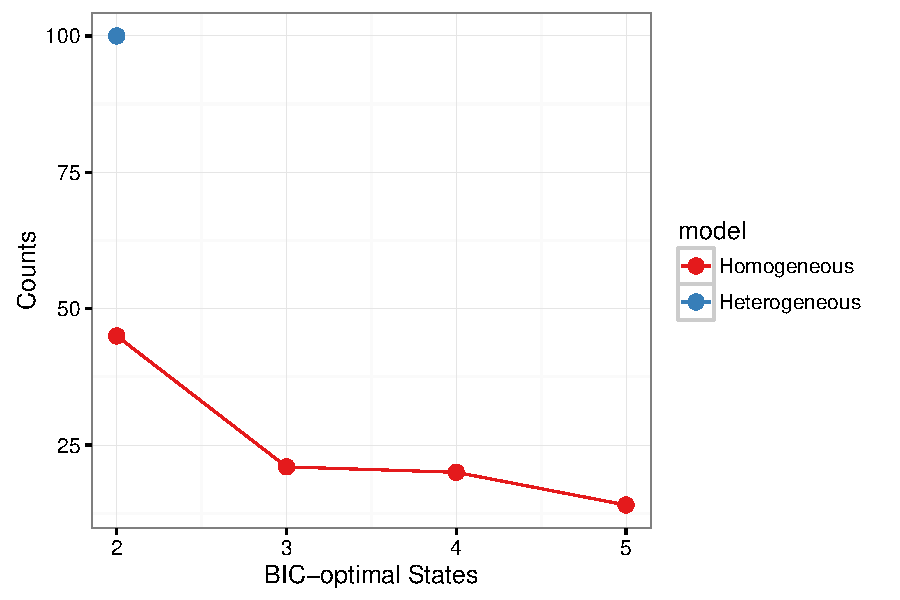
\includegraphics[width=5in]{figure/sim_results-1}
  \caption{\csentence{Simulation Results} BIC-optimal state frequency for 2-6 state HMMs with and without covariate transition on 100 two-state hidden Markov models with covariate transitioning simulations.}
      \end{figure}

  \begin{figure}[h!]
   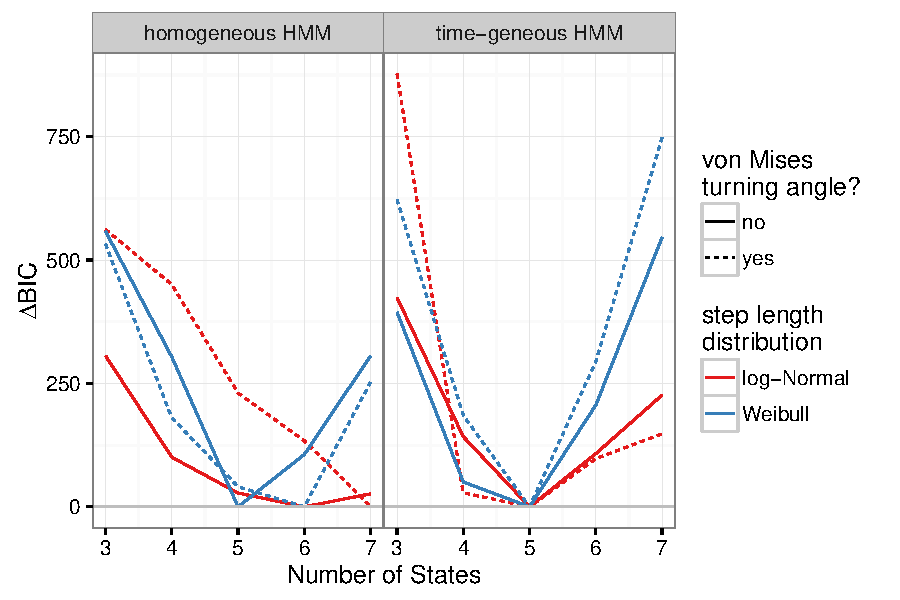
\includegraphics[width=5in]{figure/BICred_plot-1}
  \caption{\csentence{Adjusted BIC Emission Distribution Comparison} Adjusted Bayesian information criterion values for 3-7 state HMMs with different step-length distributions, with and without temporal transitions and turning angles.}
      \end{figure}
      
  \begin{figure}[h!]
   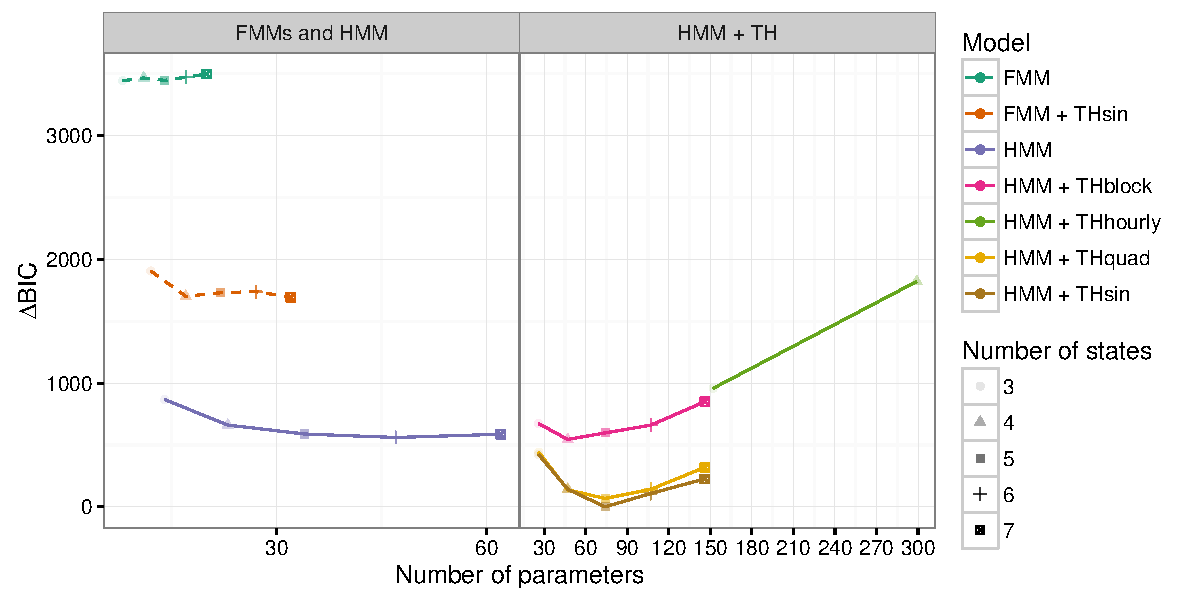
\includegraphics[width=5in]{figure/adj_BIC_comparisons-1}
  \caption{\csentence{Adjusted BIC Transition Comparison} Adjusted BIC by number of free parameters for HMM model types. The left panel shows FMM, FMM with a sin prior and HMM. The right panel shows HMMs with different temporal transitions.}
      \end{figure}
      
\begin{figure}[h!]
   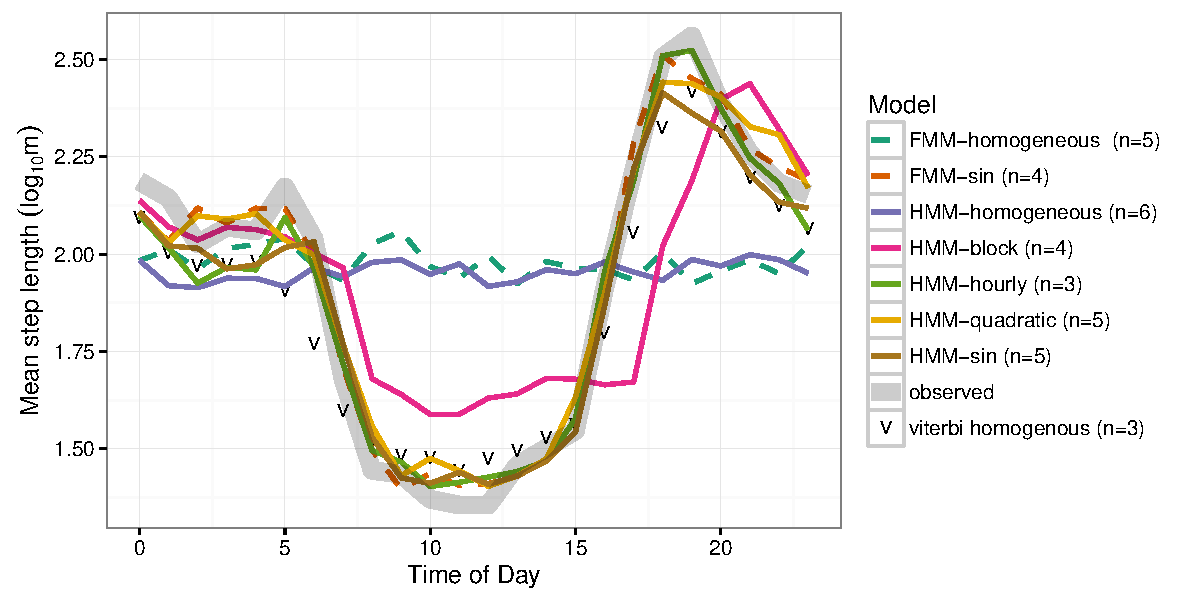
\includegraphics[width=5in]{figure/avg_step_length_by_time-1}
  \caption{\csentence{Diurnal Step Lengths Plot} Average step length by time of day observed (gray highlight), three-state HMM Viterbi predictions (V points), and all transitions type HMMs predictions (out of sample) with their respective BIC-optimal states.}
      \end{figure}
      
\begin{figure}[h!]
   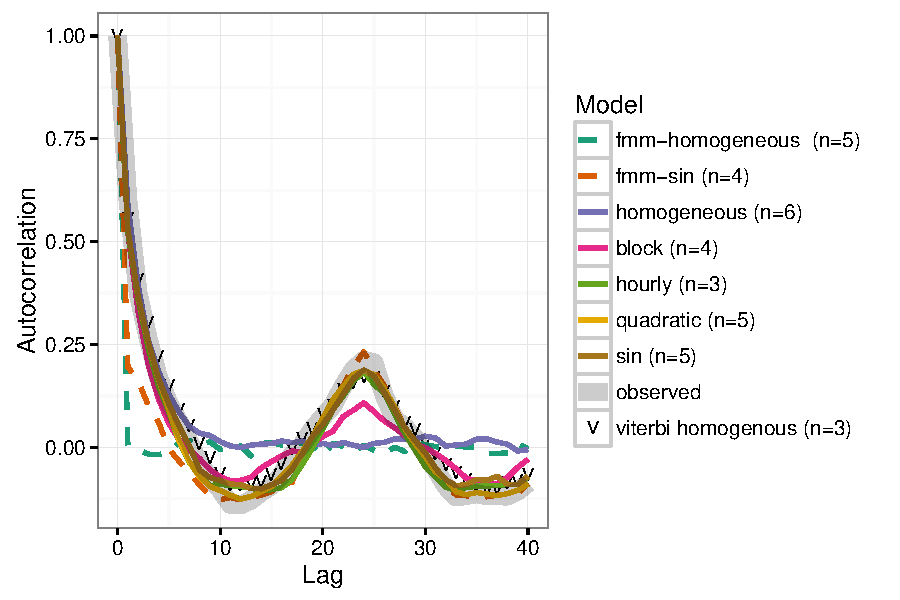
\includegraphics[width=5in]{figure/acf_plot-1}
  \caption{\csentence{Autocorrelation Plot} Autocorrelation of observed (gray highlight), three-state HMM Viterbi predictions (V points), and all transitions type HMMs predictions (out of sample) with their respective BIC-optimal states.}
      \end{figure}
      
\begin{figure}[h!]
   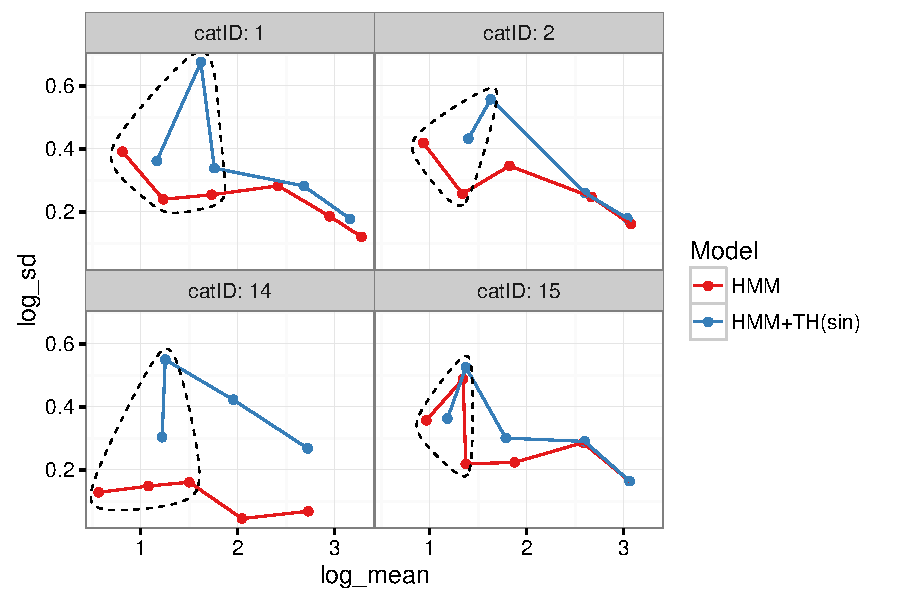
\includegraphics[width=5in]{figure/r_msdlist-1}
  \caption{\csentence{State Identification Plot} Log mean and standard deviation of BIC-optimal HMM and HMM with sinusoidal transition.}
      \end{figure}
      
\end{backmatter}
\end{document}
